\documentclass{article}

\usepackage{graphicx} % more modern
\usepackage{subfigure} 
\usepackage{amssymb}
\usepackage{amsmath}
\usepackage{amsthm}


% For citations
\usepackage{natbib}

% For algorithms
\usepackage{comment}
\usepackage{framed}
\usepackage{algorithm}
\usepackage{algorithmic}
\usepackage{amsmath}
%\usepackage{algorithmicx}
%\usepackage{algpseudocode}

\usepackage{hyperref}

\allowdisplaybreaks

\newcommand{\theHalgorithm}{\arabic{algorithm}}

\newtheorem{theorem}{Theorem}[section]
\newtheorem{lemma}[theorem]{Lemma}
\newtheorem{conjecture}[theorem]{Conjecture}
\newtheorem{proposition}[theorem]{Proposition}
\newtheorem{definition}[theorem]{Definition}
\newtheorem{corollary}[theorem]{Corollary}

\usepackage[accepted]{icml2012}  % XXX : just set temporarly to print out authors corretly.

\renewcommand{\algorithmicrequire}{\textbf{Input:}}
\renewcommand{\algorithmicensure}{\textbf{Output:}}

\begin{document} 

\icmltitle{Formulas discovery for polynomial expressions}

\icmlauthor{Wojciech Zaremba}{zaremba@cs.nyu.edu}
\icmlauthor{Karol Kurach}{kkurach@google.com}
\icmlauthor{Rob Fergus}{fergus@cs.nyu.edu}


\icmlkeywords{machine learning, optimization, automatic theorem proving, RBM, NP, Boltzmann machine}

\vskip 0.3in


\begin{abstract} We present method based on attributive grammars of automatic
  discovery relations between polynomial expressions.  Surprisingly, we found
  new fast way of approximating partition function, as well as computing exact
  values of common matrix operations like $\sum AB$ (where $A$, $B$ are
  matrices). Moreover, our method can be consider
  as a formal system in which we encourage to apply machine learning based
  reasoning methods like probabilistic programming.
\end{abstract} 

\section{Introduction} \label{introduction} 

Progress in some branches of
mathematics might be restricted by size of symbolic derivations that human can
handle.  Mathematicians can deal with expressions having up to some small
number of variables having different purposes in equations. However, there
might exists very handy relations between expressions having hundreds or
thousands of variables. We will show how task of finding equivalent
mathematical expressions can be automated. Our focus is on finding equivalent
mathematical formulas, which are faster to compute than the original one. Where
faster can be defined as (1) number of operations, or (2) computational time
for any particular computational hardware.


We propose deterministic, grammar based framework, which discovers relations between
multi-variable polynomial expressions. First, we construct an attribute grammar
-- a context-free grammar extended to contain set of attributes, introduced by
Donald Knuth \cite{knuth1968semantics}. To define the search space we use a set
context-free grammar rules representing admissible operations. By representing
the cost of every operation as a synthetized attribute (i.e. computed bottom-up from child node attributes)
we can search for formula with low time complexity.
Through linear combination of grammar elements, we find solution to desired 
expressions that we want to compute. Finally, we
show that this computation solution can be further speed up by use of standard
techniques of optimization in compiler domain. We show power of presented
approach by deriving close form, $O(n^3)$ time solutions to compute partition
function like expressions for RBMs. Presented close form solutions oppose
widespread believe that hardness of partition function computation is in its
exponential number of elements.


Finally, we look on set of generated rules as on small axiomatic system.
Presented algorithm is deterministic, finite time proof in this system.
We are excited about using machine learning for automatic reasoning, and
this subset of mathematics seem to be perfect fit for testing automatic reasoning systems.
Usually, axiomatic systems like number theory, set theory, or topology have very small
number of axioms, but their application to terms might be complex. Proofs
for such systems are difficult to represent in software, and there is no
baseline algorithms which could brute force proof by iterating over all of them in reasonable finite time.
Where in the contrary, presented here axiomatic system has very simple representation
in software, and this paper presents brute force algorithm to find proofs. 
Surprisingly, even brute force algorithm is able to find new more efficient,
computational expressions for expressions that we use.

By the time of publication we are going to release code.


\section{Related work} \label{relatedwork}


Attribute grammar, originally developed in 1968 by Knuth \cite{knuth1968semantics} in context of compiler
construction, was successfully used as a tool for design, formal specification
and implementation of practical systems. It influenced various areas of
Computer Science such as natural language processing \cite{hafiz2011modular}, \cite{starkie2002inferring}, 
definite clause grammars \cite{bratko2001prolog}, query processing \cite{koch2007attribute}, \cite{ramakrishnan1991top} and specification of algorithms \cite{bellanova1984examples}.
Thirunarayan \cite{thirunarayan2009attribute} provides a good overview of their
applications, including static analysis of programs, program translation, specifying information
extraction algorithms and optimization of datalog programs.

In our work, we focus on applying attribute grammar for optimization problem. This class
of problems was successfully addressed in range of domains: from well-known algorithmic problems 
like knapsack packing \cite{o2004solving}, through bioinformatics \cite{waldispuhl2002approximate} to music domain\cite{desainte1994using}.
We are not aware of any previous work related to discovering mathematical formulas. However,
similar concepts can be found in \cite{cheung1999attribute} where authors are searching
the space of algorithms and attributes are also computational complexity.


\section{Terminology}
Before delving into content of this work, we will establish vocabulary.


{\bf Space of matrices of polynomials} - We consider matrix of homogeneous polynomials, which we denote by $\mathcal{P}^{n \times m}_k$. Upper index indicates size of matrix, and lower indicates degree. For instance, $\begin{pmatrix} a^3 + b^3 & b^3 + bc^2 + c^3\\ cd^2 & d^3 \end{pmatrix} \in \mathcal{P}^{2 \times 2}_3$. 


{\bf Grammar} - We consider a attributive grammar on tuples (expression, computation, computational time). We refer to this tuples as literals. 


{\bf Production rules} - describes how to transform a tuple (expressions, computation, computation time), or few tuples to the new tuple. 


{\bf Expression} - Expressions are matrices of polynomials having a homogeneous degree $\alpha$. They belong to the spaces $\mathcal{P}^{n \times m}_\alpha$. Different expressions might be in different spaces, and it restricts which rules can be 
applied to literals containing such expressions. We denote them with capital characters (e.g. $\mathbb{E}$).


{\bf Computation} - Represents a computation on particular architecture or programming language. It our examples we consider Matlab as underlaying computation language. We denote them with capital, calligraphic characters (e.g. $\mathcal{C}$).


{\bf Computation Time} - It is a computation time for a particular architecture and programming language, or it can represent computation complexity. For a computation $\mathcal{C}$, we refer to its computation time as $t_{\mathcal{C}}$. 


Let's consider a literal $L = (\mathbb{E}, \mathcal{C}, t_\mathcal{C})$. $\mathbb{E}$ is a polynomial in $\mathcal{P}^{n \times m}$. $\mathcal{C}$ is a computation of this polynomial starting with a input matrices. Result of computation is a real matrix
in $\mathbb{R}^{n \times m}$, which is computed in time $t_\mathcal{C}$. This time is a time necessary to perform computation on instantiations of matrices (not computation during grammar derivation, which would involve expressions).

\section{Admissible computation as a grammars}\label{sec:grammars}

The final goal is to find a fast way of expressing target expression.
We will achieve it by developing literals in grammar (up to degree of target expression). Next, we
will look for the linear combination of obtained expressions to find how to express target expression.
We know how to compute every obtained expression, as the literal which consists of it, has also computation field.
Moreover, if there multiple literals with the same expression, we choose one with the shortest computation time.


Let's ground our approach in an example. We assume that we are interest in
finding algorithm with smallest operation complexity, and computation platform
is a Matlab.  We consider following set of operations on matrices : 

\begin{figure}
\begin{framed}
\begin{align*}
&\text{{\bf Element wise multiplication}}\\
&(\mathbb{A} \in \mathcal{P}^{n \times m}_\alpha, \mathcal{A}, t_\mathcal{A}), (\mathbb{B} \in \mathcal{P}^{n \times m}_\beta, \mathcal{B}, t_\mathcal{B}) \rightarrow \\ 
&(\mathbb{C} \in \mathcal{P}^{n \times m}_{\alpha + \beta}, \mathcal{A} .* \mathcal{B}, O(t_\mathcal{A} + t_\mathcal{B} + nm)) \\
&\mathbb{C}_{i,j} = \mathbb{A}_{i,j}\mathbb{B}_{i, j} \text{ for } i \in \{1, \dots, n\}, j \in \{1, \dots, m\} \\
&\text{{\bf Matrix multiplication}}\\
&(\mathbb{A} \in \mathcal{P}^{n \times m}_\alpha, \mathcal{A}, t_\mathcal{A}), (\mathbb{B} \in \mathcal{P}^{m \times k}_\beta, \mathcal{B}, t_\mathcal{B}) \rightarrow \\ 
&(\mathbb{C} \in \mathcal{P}^{n \times k}_{\alpha + \beta}, \mathcal{A} * \mathcal{B}, O(t_\mathcal{A} + t_\mathcal{B} + nmk)) \\
&\mathbb{C}_{i,k} = \sum_{k = 1}^m \mathbb{A}_{i,k}b_{k, j} \text{ for } i \in \{1, \dots, n\}, j \in \{1, \dots, m\} \\
&\text{{\bf Columns marginalization}}\\
&(\mathbb{A} \in \mathcal{P}^{n \times m}_\alpha, \mathcal{A}, t_\mathcal{A}) \rightarrow \\ 
&(\mathbb{C} \in \mathcal{P}^{n \times 1}_\alpha, sum(\mathcal{A}, 2), O(t_\mathcal{A} + nm)) \\
&\mathbb{C}_{i, 1} = \sum_{j = 1}^m \mathbb{A}_{i, j} \text{ for } i \in \{1, \dots, n\}\\
&\text{{\bf Rows marginalization}}\\
&(\mathbb{A} \in \mathcal{P}^{n \times m}_\alpha, \mathcal{A}, t_\mathcal{A}) \rightarrow \\ 
&(\mathbb{C} \in \mathcal{P}^{1 \times m}_\alpha, sum(\mathcal{A}, 1), O(t_\mathcal{A} + nm)) \\
&\mathbb{C}_{1, j} = \sum_{i = 1}^m \mathbb{A}_{i, j} \text{ for } j \in \{1, \dots, m\}\\
&\text{{\bf Columns repetition}}\\
&(\mathbb{A} \in \mathcal{P}^{n \times 1}_\alpha, \mathcal{A}, t_\mathcal{A}) \rightarrow \\ 
&(\mathbb{C} \in \mathcal{P}^{n \times m}_\alpha, repmat(\mathcal{A}, 1, m), O(t_\mathcal{A} + nm)) \\
&\mathbb{C}_{i, j} = \mathbb{A}_{i, 1} \text{ for } i \in \{1, \dots, n\}\\
&\text{{\bf Rows repetition}}\\
&(\mathbb{A} \in \mathcal{P}^{1 \times m}_\alpha, \mathcal{A}, t_\mathcal{A}) \rightarrow \\ 
&(\mathbb{C} \in \mathcal{P}^{n \times m}_\alpha, repmat(\mathcal{A}, n, 1), O(t_\mathcal{A} + nm)) \\
&\mathbb{C}_{i, j} = \mathbb{A}_{1, j} \text{ for } j \in \{1, \dots, m\}\\
&\text{{\bf Entry repetition}}\\
&(\mathbb{A} \in \mathcal{P}^{1 \times 1}_\alpha, \mathcal{A}, t_\mathcal{A}) \rightarrow \\ 
&(\mathbb{C} \in \mathcal{P}^{n \times m}_\alpha, repmat(\mathcal{A}, n, m), O(t_\mathcal{A} + nm)) \\
&\mathbb{C}_{i, j} = \mathbb{A}_{1, 1} \text{ for } i \in \{1, \dots, n\}, j \in \{1, \dots, m\}\\
&\text{{\bf Transposition}}\\
&(\mathbb{A} \in \mathcal{P}^{n \times m}_\alpha, \mathcal{A}, t_\mathcal{A}) \rightarrow \\ 
&(\mathbb{C} \in \mathcal{P}^{m \times n}_\alpha, A', O(t_\mathcal{A} + nm)) \\
&\mathbb{C}_{j, i} = \mathbb{A}_{i, j} \text{ for } i \in \{1, \dots, n\}, j \in \{1, \dots, m\} \\
\end{align*}
\caption{Set of rules for attributive grammar. There is always finite number of literals up to degree $\alpha$.}
\end{framed}
\label{rules}
\end{figure}

% XXX : Speak somewhere about mutliplicative constant.

To find any (or cheapest) way of computing target expression $\mathbb{T}$ of degree $k$, we proceed as follows : 
\begin{itemize}
\item develop grammar to obtain all possible literals up to degree $k$. It gives rise to finite number of literals.
\item if there are multiple way of computing the same expression, choose one with shortest time
\item find linear combination of expressions which is equal the target expression $\mathbb{T}$ (this relation is a symbolic relation, which is valid for any assignment of symbols). While solving this linear set of systems, choose solution with
smallest sum of computation times.
\item apply optimization like subexpression elimination, and exploit distributive property of multiplication in order to decrees final computational time of $Y$. This step is optional, and it won't decrease computational complexity.
\end{itemize}

Aforementioned algorithm can be expressed with a psedocode \ref{pseudocode}.

\begin{algorithm}
\caption{Find computation for expression}
\begin{algorithmic} 
\REQUIRE Target expression $\mathbb{T}$, initial expression $W$, $Rules$ = \{$R_1, \dots, R_n$\}, maximum degree of polynomials $k$
\ENSURE Computation $\mathcal{C}$ of expression $\mathbb{T}$.
\STATE Initialize set $\mathbb{S}$ of all admissible literals with $(W, \mathcal{W}, t_W)$
\WHILE{$\mathbb{S}$ grows}
\FORALL{literal $L \in \mathbb{S}$}
\FORALL{rule $R \in Rules$}
\STATE $L' \gets$ Apply rule $R$ to $L$
\IF {degree($L'$) $>$ $k$}
  \STATE \textbf{continue}
\ENDIF
\STATE \emph{// If expression not yet in $\mathbb{S}$ or it can be}
\STATE \emph{// computed faster add it.}
\IF {$L'.expr \not\in \mathbb{S}$ \textbf{or} $L'.time < S[L'].time$}
  \STATE Add $L'$ to $\mathbb{S}$
\ENDIF
%\IF {$L'.expression \in \mathbb{S}$ }
%	\IF {$L'.computation\_time$ faster than for previous expression in $\mathbb{S}$} 
%		\STATE Add $L'$ to $\mathbb{S}$
%	\ENDIF
%\ELSE[$L'$ contains a new, unseen expression]
%	\STATE Add $L'$ to $\mathbb{S}$
%\ENDIF
\ENDFOR
\ENDFOR
\ENDWHILE
\STATE Find linear combination of expressions from literals stored in $\mathbb{S}$ to express $\mathbb{T}$
\STATE Run optimizer
\end{algorithmic}
\label{pseudocode}
\end{algorithm}


\subsection{Linear combination}
We look for linear combination of generated expressions in our literals, which is equal to the
target expression. There is few possible scenarios. There might be \emph{no solution} at all. 
Then our linear solver will indicate it, which means that target expression
is out of scope for computation defined by our grammar. There might be \emph{multiple solutions} (case
with a \emph{single solution} is very uncommon). Then we should look for linear combination
with the smallest cost (computational time). 
This is essentially integer programing problem, or knapsack problem, which 
are NP-complete. However, it is enough for us to get approximated solution, which can be easily
obtained with linear solver.


Experiments suggest to minimize number of coefficients as well. It helps to rule out
non-integer coefficient values, which might cause numerical errors. 


\subsection{Optimization}

Application of grammar rules gives rise to a tree. Moreover, last step of
combining elements together can be also consider as adding plus node to the
tree. Optimization procedures are applied recursively to tree branches, and
transform them to more efficient computationally equivalents. We used common in
compiler literature optimization techniques like subexpression elimination.
Further, we optimized our symbolic tree by exploiting (1) distributive, and (2)
associative properties of multiplication, and addition (together with
commutative property for addition).

\subsection{Grammars}
Presented attributive grammar is just a example of grammar which is finite
and seems to solve many problems. However, one could extend it with 
other operations like e.g. inverse of matrix. Moreover, one could exploit
rules which could discover recurrences (to be able to discover discreet Fourier transform, or
Strassen algorithm for fast matrix multiplication).

\subsection{Representation of expressions}

Expressions are defined as belonging to $\mathcal{P}^{n \times m}_\alpha$. There are various
ways how they can be represented in software. This representation is crucial, and has consequences in
 correctness of solution (due to numerical errors), and computation speed.

\subsubsection{Evaluation of polynomials in $\mathbb{R}$}
As expressions correspond to the matrices of polynomials, one could just record their values
for many random numbers. If number of evaluations is large enough, then polynomials can be
recovered based on such values. Or even one could keep this representation over entire 
computation without recovering polynomials, but deriving final relation between polynomials (that's what we implemented).
It turns out, that this methods is numerically unstable
, and for polynomials of degree $k \geq 3$, it is not able to produce solutions, even if there are some.

Nice part about this representation is that operations like element-wise matrix multiplication, addition of matrices, etc.
correspond just to the same operations in our representation (of same computational cost). i.e. For element-wise multiplication of matrices of expressions, we
have to perform element-wise multiplication of real numbers (on multiple instances of random values assignments).

\subsubsection{Symbolic representation}
Expressions can represented as matrices of polynomials. Every expression has list of coefficients and monomials, which it constitutes of.
This representation is exact, and gives us guarantees on correctness. However,
it might be quite slow. For instance, if two polynomials, which we want to multiply constitutes of 1000 coefficients, then
it takes $\sim 1mln.$ operations. We have implemented expressions in such representation, and it allowed us
to find patterns for polynomials up to degree $4$ (above degree $4$ it was consuming too much time).

This solution guarantees correctness, and it is easiest to debug.

\subsubsection{Evaluation of polynomials in $\mathbb{Z}_p$}
We use similar strategy as in case of looking into evaluations of polynomials in $\mathbb{R}$. However, in order
to avoid numerical errors, we replace real number computation with computation in $\mathbb{Z}_p$ group (for large prime number $p$). This
guarantees that all the results of the computation are represented correctly (there is no round off errors on integers). Nonetheless, there are few potential
issues. We could have two different expressions being represented the same way (conflict of representations). In the
real setting, we haven't run into this problem. Moreover, all the final coefficients after applying linear solver are
accurate up to $p$ offset. This turns out also not to be an issue. For all coefficients above $\frac{p}{2}$, we subtract $p$. 
This way all final coefficients are in the range $[-\frac{p}{2}, \frac{p}{2}]$. We have verified that such solutions are correct
(it can be considered as prior on magnitude of coefficients). 

This solution is fastest, and most reliable. However, it is difficult to debug.


\section{Partition function of RBM} \label{partitionfunction}
Algorithm presented in Section
\ref{sec:grammars} allows to find concise formulas for polynomial expressions.
However, many interesting functions are outside of this family.  Instead of it,
we are going to consider Taylor expansion of desired function, and we will
derive close form fast formula for it.

Let's denote by $g(f, W)$ generalization of partition function. 
$g$ is a functional, and it takes as argument a function $f : \mathbb{R} \rightarrow \mathbb{R}$,
and weights $W$. It is defined as follow : 

\begin{gather*}
g(f, W) = \sum_{v \in \{0, 1\}^n, h \in \{0, 1\}^m} f(v^TWh) \\
f : \mathbb{R} \rightarrow \mathbb{R}\\
W \in \mathbb{R}^{n \times m}
\end{gather*}

We consider computation of $g(x \rightarrow x^k, W)$ for a given $k$ for any $W
\in \mathbb{R}^{n \times m}$, for any $n, m$. Potentially, if we would be able
to compute $g(x \rightarrow x^k, W)$ for $k = 1, \dots, K$, than partition
function for finite energy $v^TWh < C$ could be approximated arbitrarily well.
This is consequence of expressing $e^{x}$ as finite sum approximation through
Taylor expansion.

\subsection{Low degree examples} In order to present how our algorithm works,
we will manually derive fast computation procedure for $g(x \rightarrow k, W)$.
However, this can be done manually only for very small $k = 1, 2$. 


\subsubsection{$g(x \rightarrow x, W)$} Let's consider function $f(x) = x$. We
will show that function $g(x \mapsto x, W)$ is computable in $O(nm)$ time
(linear with respect to number of entries in $W$ matrix).
 
\begin{gather*}
	g(x \mapsto x, W) = \sum_{v \in \{0, 1\}^n, h \in \{0, 1\}^m} v^TWh
\end{gather*}

Entry $w_{i,j}$ in above sum is counted only if $v_i = 1$ and $h_j = 1$. Other variables
$v_1, \dots v_{i-1}, v_{i+1}, \dots v_n$ and $h_1, \dots h_{i-1}, h_{j+1}, \dots h_m$ can be 
assigned arbitrary. Number of arbitrary assignments of remaining variables is $2^{n + m - 2}$. 
This concludes that 

\begin{gather*}
	\sum_{v \in \{0, 1\}^n, h \in \{0, 1\}^m} v^TWh = 2^{n + m - 2}\sum_{i = 1, \dots, n, j = 1, \dots, m} W_{i, j}
\end{gather*}
, which is the close form solution for sum over exponentially many elements.

\subsubsection{$g(x \rightarrow x^2, W)$}

We are interest in computing following expression : 
\begin{gather*}
	g(x \mapsto x^2, W) = \sum_{v \in \{0, 1\}^n, h \in \{0, 1\}^m} (v^TWh)^2
\end{gather*}

There are multiple second order monomials that emerge: 

\begin{itemize}
	\item $w_{i,j}^2$ - present iff $v_i = 1, h_j = 1$. Appears $2^{n + m - 2}$ times.
	\item $w_{i,j} w_{i, k}, j \neq k$ - present iff $v_i = 1, h_j = 1, h_k = 1$. Appears $2^{n + m - 3}$ times.	
	\item $w_{i,j} w_{k, j}, i \neq k$ - present iff $v_i = 1, v_k = 1, h_j = 1$. Appears $2^{n + m - 3}$ times.
	\item $w_{i,j} w_{k, l}, i \neq k, j \neq l$ - present iff $v_i = 1, v_k = 1, h_j = 1, h_l = 1$. Appears $2^{n + m - 4}$ times.			
\end{itemize}
We encode above quantities in a vector, which indicate how many times particular monomials 
appear. Vector expressing this relation for $g(x \mapsto x^2, W)$ is $(2^{n + m - 2}, 2^{n + m - 3}, 2^{n + m - 3}, 2^{n + m - 4})$


Let us consider following expressions : 
\begin{itemize}
 \item $\sum_{i = 1, \dots, n, j = 1, \dots m} W_{i, j}^2$ encodes $(1, 0, 0, 0)$. 
 \item $(\sum_{i = 1, \dots, n, j = 1, \dots m} W_{i, j})^2$ encodes $(1, 1, 1, 1)$.
 \item $\sum_{i = 1, \dots, n}(\sum_{j = 1, \dots, m} W)^2$ encodes $(1, 1, 0, 0)$. 
 \item $\sum_{j = 1, \dots, m}(\sum_{i = 1, \dots, n} W)^2$ encodes $(1, 1, 0, 0)$. 
\end{itemize}
 
 By solving linear equation :
 \begin{equation}
 \begin{pmatrix} 
  1 & 1 & 1 & 1 \\ 
  0 & 1 & 1 & 0 \\ 
  0 & 1 & 0 & 1 \\ 
  0 & 1 & 0 & 0 \\     
\end{pmatrix}t = 2^{n + m - 4}\begin{pmatrix} 
  2^{2}\\ 
  2^{1}\\ 
  2^{1}\\ 
  2^{0}\\     
\end{pmatrix} \\
 \end{equation}

One can find that 
\begin{align*}
	&g(x \mapsto x^2, W) = 2^{n + m - 4} \\ 
 &\Big(\sum_{i = 1, \dots, n, j = 1, \dots m} W_{i, j}^2 + (\sum_{i = 1, \dots, n, j = 1, \dots m} W_{i, j})^2 + \\
 &\sum_{i = 1, \dots, n}(\sum_{j = 1, \dots, m} W)^2 + \sum_{j = 1, \dots, m}(\sum_{i = 1, \dots, n} W)^2 \Big)\\
\end{align*}

Above derivation is still in scope of human skills. However, manual derivation
of $g(x \mapsto x^k, W)$ for further $k > 2$  seems to be a feet. Our algorithm
is able to find such complex computational patterns automatically. 

\subsubsection{$g(x \rightarrow x^3, W)$}
Manual derivation for $k = 3$ seems to be a hard task. We present here all derived computations in
for expressions in $\mathcal{P}^{1 \times 1}_3$. 

\begingroup
    \fontsize{8pt}{12pt}\selectfont
\begin{itemize}
	\itemsep-5px 
	\item \begin{verbatim} sum(sum(W, 2), 1) \end{verbatim}
	\item \begin{verbatim} (sum(sum(W, 2), 1) .* sum(sum(W, 2), 1)) \end{verbatim}
	\item \begin{verbatim} sum((sum(W, 1) .* sum(W, 1)), 2) \end{verbatim}
	\item \begin{verbatim} sum(sum(((repmat(sum(W, 2), [1, m]) .*  ...
		repmat(sum(W, 1), [n, 1])) .* W), 2), 1) \end{verbatim}
	\item \begin{verbatim} sum((sum(W, 1) .* (sum(W, 1) .* sum(W, 1))), 2) \end{verbatim}
	\item \begin{verbatim} sum((sum(W, 2) .* sum(W, 2)), 1) \end{verbatim}
	\item \begin{verbatim} sum((sum(W, 2) .* (sum(W, 2) .* sum(W, 2))), 1) \end{verbatim}
	\item \begin{verbatim} sum(sum((W .* W), 2), 1) \end{verbatim}
	\item \begin{verbatim} sum(sum(W, 2), 1) .^ 3 \end{verbatim}
	\item \begin{verbatim} sum(sum((repmat(sum(W, 1), [n, 1]) .^ 2  .* ...
		 (repmat(sum(W, 2), [1, m]))), 1), 2) \end{verbatim}
	\item \begin{verbatim} sum((sum(W, 1) .* sum((W .* W), 1)), 2) \end{verbatim}
	\item \begin{verbatim} (sum(sum(W, 2), 1) .* sum(sum((W .* W), 2), 1)) \end{verbatim}
	\item \begin{verbatim} sum(sum((repmat(sum(W, 2), [1, m]) .^ 2 .* ...
		repmat(sum(W, 1), [n, 1]))), 2), 1) \end{verbatim}
	\item \begin{verbatim} sum((sum(W, 2) .* sum((W .* W), 2)), 1) \end{verbatim}
	\item \begin{verbatim} sum(sum((W .* (W .* W)), 2), 1) \end{verbatim}
\end{itemize}
\endgroup


Expression $g(x \rightarrow x^3, W)$ can be computed exactly with :

\begingroup
    \fontsize{8pt}{12pt}\selectfont
\begin{verbatim}
((((sum(sum(W, 2), 1) .* (sum(sum(W, 2), 1) ...
.* sum(sum(W, 2), 1)))) + ((sum(sum(W, 2), 1) ...
.* sum((sum(W, 2) .* sum(W, 2)), 1)) .* 3) ...
+ ((sum(sum(W, 2), 1) ...
.* sum(sum((W .* W), 2), 1)) .* 3) ...
+ ((sum(sum(W, 2), 1) .* sum((sum(W, 1) ...
.* sum(W, 1)), 2)) .* 3) + (sum((sum(W, 2) ...
.* sum((W .* repmat(sum(W, 1), ...
[n, 1])), 2)), 1) .* 6))) / 64;
\end{verbatim}
\endgroup


\section{Experiments}

We present various mathematical expressions, which can be computed more efficiently
than initial formulation would suggest. This section is finalized with  
approximations of partition function. 

\subsection{Snippets}

There are given matrices $A \in \mathbb{R}^{n \times m}$, $B \in \mathbb{R}^{m \times k}$. 
Goal is to compute 
\begin{align*}
	\sum AB = \sum_{i = 1}^n \sum_{k = 1}^m \sum_{j = 1}^k A_{i, k} B_{k, j} 
\end{align*}
Naive algorithm would take $O(nmk)$ time. However, we have found with our framework 
computation giving the same expression in time O(n(k + m)) :

\begin{verbatim}
	sum(sum(A .* repmat(sum(B, 2), [1, n])'))
\end{verbatim}

Empirical tests indicate that aforementioned computation is indeed faster (Figure \ref{ab}).

\begin{figure}[h]
\centering
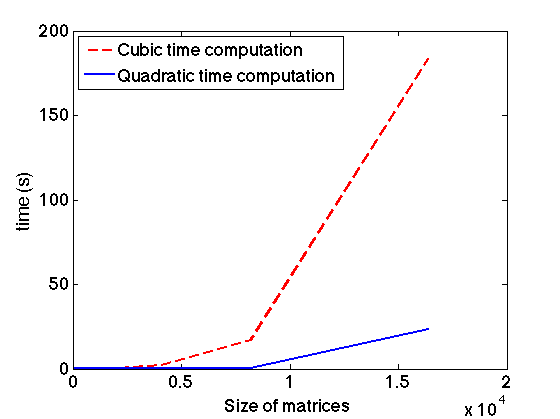
\includegraphics[scale=0.3]{img/ab.png}
\caption{Computation time for $\sum AB$ using standard algorithm vs using inferred optimal algorithm.}
\label{ab}
\end{figure}


Similarly, we found quadratic time computation instead of cubic for similar expressions like : 
\begin{align*}
	\sum ABC\\
	\sum ABCD\\
	\sum AA^T\\
	\sum AA^TA\\
\end{align*}

One could automatically analyze large code repositories to find other expressions, which are computed inefficiently. 
Our optimization rules could be placed into compilers.

\subsection{Partition function approximation}

As we shown in Section \ref{partitionfunction}, we can manually find $O(n^2)$ computation of $g(x \rightarrow x^k, W)$ for $k = 1, 2$ 
instead of native exponential time computation. By use of
our framework, we found rules for $k = 3, 4, 5$ (however for $k = 4, 5$ we found only computation in $O(n^3)$ time). 
Finding computation for higher degree polynomials is expensive.
Table \ref{grammars} shows time necessary to
generate all the rules. It is worth to note, that grammar can be evaluated just once, and the resulting coefficients can 
be stored. Process of partition function approximation involves step of computation discovery only once. However, due to limited computation power
we analyzed only powers $k \leq 5$. As we noted in Section \ref{agenda}
it is extremely important and interesting to find pattern how to generate $g(x \rightarrow x^k, W)$ for $k \geq 6$.


Table \ref{eval} shows number of terms necessary to derive $g(x \rightarrow x^k, W)$ for various $k$. Plot \ref{approximations} shows 
how well partition function is approximated with finite Taylor expansion. Finally, plot \ref{time_approx} 
compares computation time of derived rules to the computation time of naive exponential time algorithm.

\begin{table}
\tiny
\centering
\begin{tabular}{|l||l|l|}
\hline\hline
Order & Size of grammar & Computation time (s) \\
\hline\hline
2 & 5 & 17 \\
3 & 15 & 188 \\
4 & 48 & 2535\\
5 & 139 & 31320 \\
\hline
\end{tabular}
\caption{Table summarizes size and computational time for grammars of specific degree.}
\label{grammars}
\end{table}

\begin{table}
\tiny
\centering
\begin{tabular}{|l|l|l|}
\hline\hline
Order & Number of terms & Complexity \\
\hline\hline
2 & 4 & $O(n^2)$\\
3 & 5 & $O(n^2)$\\
4 & 21 & $\mathbf{O(n^3)}$\\
5 & 30 & $\mathbf{O(n^3)}$\\
\hline
\end{tabular}
\caption{Table summarizes complexity of computation of $g(x \rightarrow x^k, W)$.} 
\label{eval}
\end{table}

\begin{figure}[h]
\centering
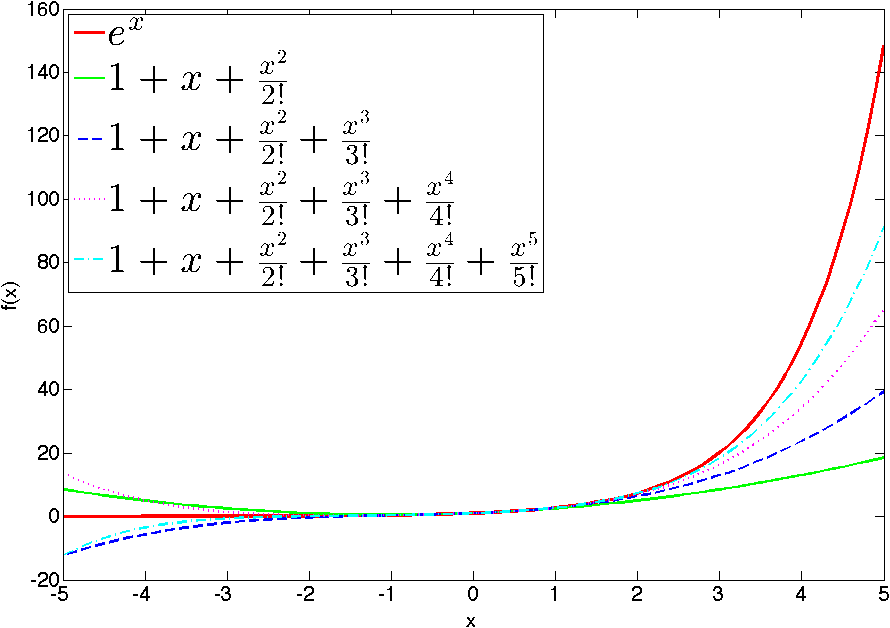
\includegraphics[scale=0.2]{img/approximations.png}
\caption{Comparison of approximations with various number of Taylor terms.}
\label{approximations}
\end{figure}



\begin{figure}[h]
\centering
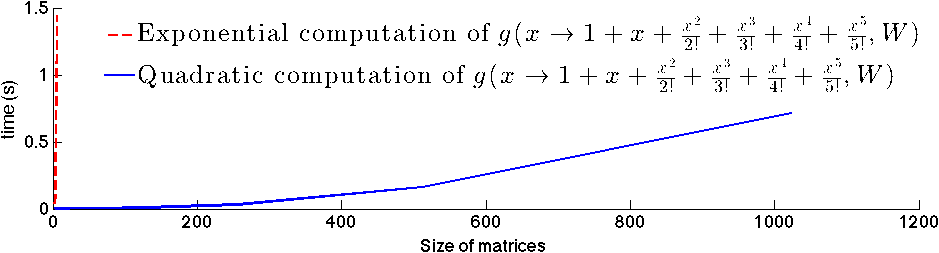
\includegraphics[scale=0.24]{img/time_approx.png}
\caption{Comparison of computation time for naive exponential time algorithm vs our optimized derivation.}
\label{time_approx}
\end{figure}

\section{Computation generalization}\label{agenda}

Presented in this paper method is a brute force over all possible computations, 
which could lead to the target result. It seems to work reasonably well
for polynomials of small degrees $k \leq 5$, however for larger powers 
brute force methods seems to fail. One of major goals of this paper is to
bring a small subset of mathematics, which has tractable brute force automatic proving
system. We look forward to extend this brute force methods to more intelligible approaches, which
could learn based on rules for smaller powers, how to solve problem for larger powers. This would
have two-fold implications in machine learning. Firstly, it would bring machine learning techniques
to the area of automatic theorem proving, which another domain of human intelligence after perception
of vision, or hearing. Secondly, solution to the problem of partition function approximation
could have consequences in unsupervised learning of RBMs, deep Bolzmann machines, and deep
belief networks. 

\section{Conjecture on hardness of partition function approximation}

We present our believes on hardness of approximation of partition function. 
We were not able to prove, or disprove conjectures presented in this chapter.
\begin{conjecture}
Linear combination of terms for a matrix $W$ generated by use of rules defined on Figure \ref{rules}.
consists of $g(x \rightarrow x^k, W)$. Moreover, size of generated grammar
up to degree $k$ is exponential in $k$.
\label{simple}
\end{conjecture}

Corollary and all implications assumes that Conjecture \ref{simple} is valid.

\begin{corollary}
	$g(x \rightarrow k, W)$
	can be computed in exponential time in $k$, but in $O(n^3)$ time with respect to size of $W$ ($W$ is of size $n \times n$).
\end{corollary}

\begin{lemma}
	For $x < C$, $e^x$ can be approximated up to $\epsilon$ accuracy in log scale with $\frac{Ce}{\epsilon}$ terms. 
\end{lemma}
\begin{proof}

For every $x < C$ there exists $t < x$, such that :  
\begin{align*}
	e^x = 1 + \frac{x}{1!} + \frac{x^2}{2!} + \dots + \frac{x^{k - 1}}{(k - 1)!} + \frac{x^k}{k!}e^t
\end{align*}
This implies
\begin{align*}
	|e^x - (1 + \frac{x}{1!} + \frac{x^2}{2!} + \dots + \frac{x^{k - 1}}{(k - 1)!}) | < \frac{C^k}{k!}e^C \\
	\sim \exp(n\log{C} + C - k\log{k} + k) < \epsilon
\end{align*}

We require that 
\begin{align*}
	k (1 + \log{C} - \log{k}) < \log{\epsilon} - C \\ 
	k (\log{Ce} - \log{k}) < \log{\epsilon} - C
\end{align*}

Let's assume, that $\log{\epsilon} < -1$, and $1 - Ce < -C$. 
Clearly, this inequality is fulfilled for $k > \frac{Ce}{\epsilon}$ :
\begin{align*}
	\frac{Ce}{\epsilon} (\log{Ce} - \log{\frac{Ce}{\epsilon}}) < \log{\epsilon} - C \\
	\frac{Ce}{\epsilon} \log{\epsilon} < \log{\epsilon} - C\\
	C < \log{\epsilon}(1 - Ce)
\end{align*}

This implies that for bounded by $C$ energy of RBMs, we can do up to $\epsilon$ approximation of partition function (in log scale) by using
$\frac{Ce}{\epsilon}$ terms of Taylor approximation. This algorithm assumes Conjecture \ref{simple} has complexity
$O(2^{\frac{Ce}{\epsilon}}n^3)$.

\end{proof}


\section{Discussion and future work}
We have presented automatic method of polynomial formulas discovery. Method itself is novel, as well 
as derived results of partition function approximation are unexpected.
There are three major directions of future research. First, concerns with computation of partition function,
its derivatives, using approximation for learning, 
approximations of deep Bolzmann machine, optimization of derived formulas, and 
understanding mathematical principles behind formulas derived by our programs. Second, is in 
learning how to generalize computation, and replace current brute force process with something more
intelligent. E.g. We could generalize computation of $g(x \rightarrow x^k, W)$ for $k = 1, \dots, 5$ to
$k > 5$. Finally, the third direction are real-world applictions of this framework on large code
databases. We could automatically detect parts of code with expressions that have suboptimal time complexity
and replace them. 



\nocite{*}
\bibliography{bibliography}
\bibliographystyle{icml2012}

\end{document} 

